\subsection{Réseaux dans leurs contextes}
\begin{itemize}
\item réseau social : similitude entre amis (on voudrait mettre ces similitudes dans le réseau)
\item réseau d'affiliation social \includegraphics[scale=0.05]{images/21_Sim.png} qui permet d'expliquer les similitudes
	\begin{itemize}
	\item personnes en contact
	\item points d'intérêts communs
	\end{itemize}
\end{itemize}

\vspace{1ex}
\textbf{Idée générale}

\begin{figure}[!ht]
	\centering
	\includegraphics[scale=0.4]{images/21_IdeeGenerale.png}
\end{figure}

\subsection*{Exemples}
Il y a trois formes de fermeture :

\begin{figure}[!ht]
\begin{minipage}{\linewidth}
    \centering
    \begin{minipage}[t]{0.3\linewidth}
        \centering
        \includegraphics[width=\linewidth]{images/21_FermetureTriadique.png}
        \caption{Fermeture triadique}
    \end{minipage}
    \vrule
    \begin{minipage}[t]{0.3\textwidth}
        \centering
        \includegraphics[width=\linewidth]{images/21_FermetureFocale.png}
        \caption{Fermeture focale}
    \end{minipage}
    \vrule
    \begin{minipage}{0.3\textwidth}
        \centering
        \includegraphics[width=\linewidth]{images/21_FermetureAdhesion.png}
        \caption{Fermeture d'adhésion}
    \end{minipage}
\end{minipage}
\end{figure}

\section{La formation des liens (selon les 3 approches)}
Grâce à l'accès aux informations et aux outils d'analyse de réseau social, on peut observer les liens de plusieurs façons.
\begin{itemize}
\item On a des données réelles via les réseaux sociaux
\item On a plus facilement un accès direct aux graphes qu'avant.
\item On peut mesurer empiriquement le taux de création des liens en fonction du nombres d'amis communs.
\end{itemize}

\subsection{Algorithme}
\begin{enumerate}
\item Capture à deux instants différents le réseau (appelons ces deux graphes (1) et (2))
\item Pour chaque entier "k" plus grand ou égal à 0 :
\begin{itemize}
	\item On identifie les paires de noeuds qui ont "k" amis en communs dans (1)
\end{itemize}
\item On regarde dans (2) si pour chaque paire un lien s'est formé
\end{enumerate}
=> On calcule T(k) = fraction des paires qui ont formé un lien

\subsection{Modèle pour expliquer ce résultat (fermeture triadique)}
Si on prend deux personnes : s'il y a 1 ami en commun, il y a une probabilité "p" qu'un lien se forme.

Quelle est la probabilité pour "k" amis en commun ?

\paragraph*{}
La probabilité qu'aucun lien se forme quand il y a un ami en commun est de $(1-p)$.\\
On en déduit que pour "k" amis en commun, la probabilité est de $ (1-p)^{k}$\\
Dès lors, la probabilité qu'au moins 1 lien se forme pour k amis en commun est de $ 1-(1-p)^{k}$. C'est ce qui est égal à T(k).

\begin{figure}[!ht]
    \centering
    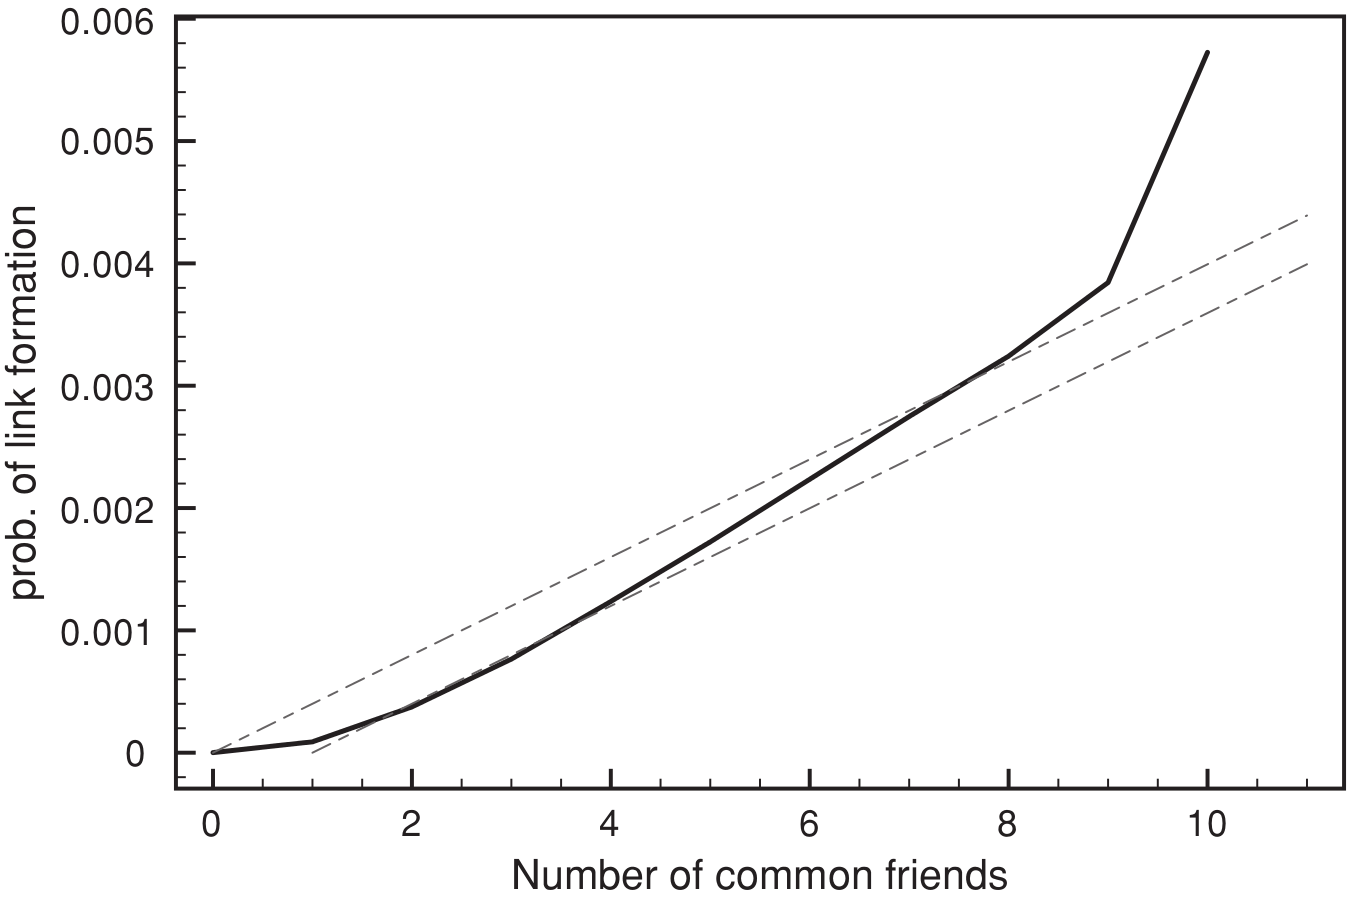
\includegraphics[width=0.8\linewidth]{images/21_emailFriends.png}
    \caption{Quantification des effets de la fermeture triadique dans un
        ensemble d'emails. La courbe déterminée à partir des données est
        une ligne noire continue. Les lignes en pointillés montrent la
        comparaison avec les probabilités depuis deux modèles simples
        dans lesquels les amis en communs fournissent des probabilités
    indépendantes de formation de lien}
    \label{emailFriends}
\end{figure}

On voit sur la figure \ref{emailFriends} (fermeture triadique) que la probabilité qu'un lien se forme augmente exponentiellement avec le nombre d'amis en commun.

\paragraph{Attention !}
Le comportement et donc les calculs sont différents pour la fermeture focale et d'adhésion !

\begin{figure}[!ht]
    \centering
    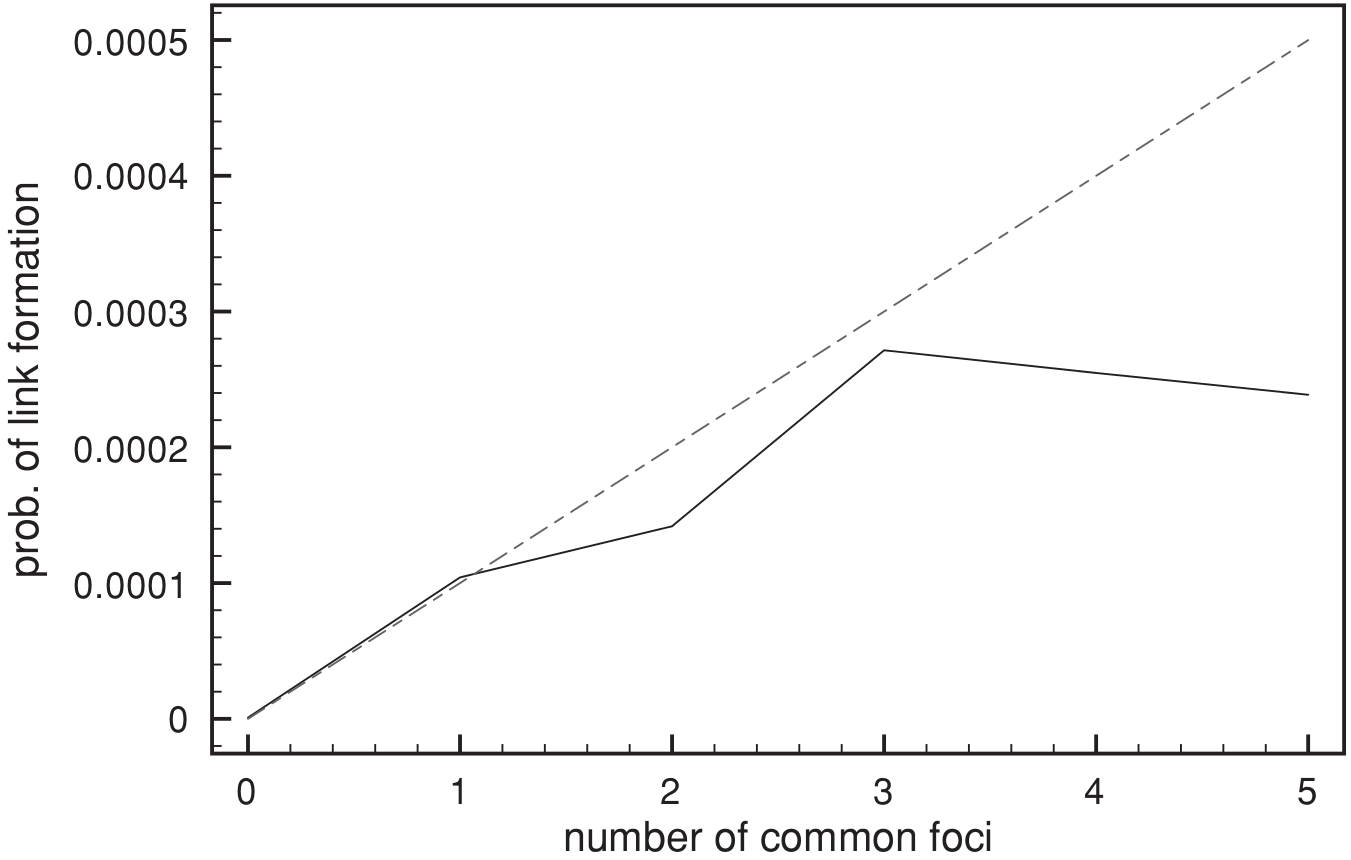
\includegraphics[width=\textwidth]{images/21_pointsCommuns.png}
    \caption{Quantification des effets d'une fermeture focalse dans un
        ensemble d'emails. A nouveau, la courbe déterminée à partir des
        données est une ligne continue, alors que la ligne en pointillés
    fournit une comparaison par rapport à une base simple.}
    \label{pointsCommuns}
\end{figure}

La figure \ref{pointsCommuns} (fermeture focale) nous montre que dans le cas où l'on considère le nombre d'intérêts en commun (ici, des cours), on arrive à un certains moment à saturation. Augmenter le nombre de points d'intérêts communs n'augmente plus la probabilité de création d'un lien à partir d'un certain point (ici 3 cours en communs).

\begin{figure}[!ht]
    \centering
    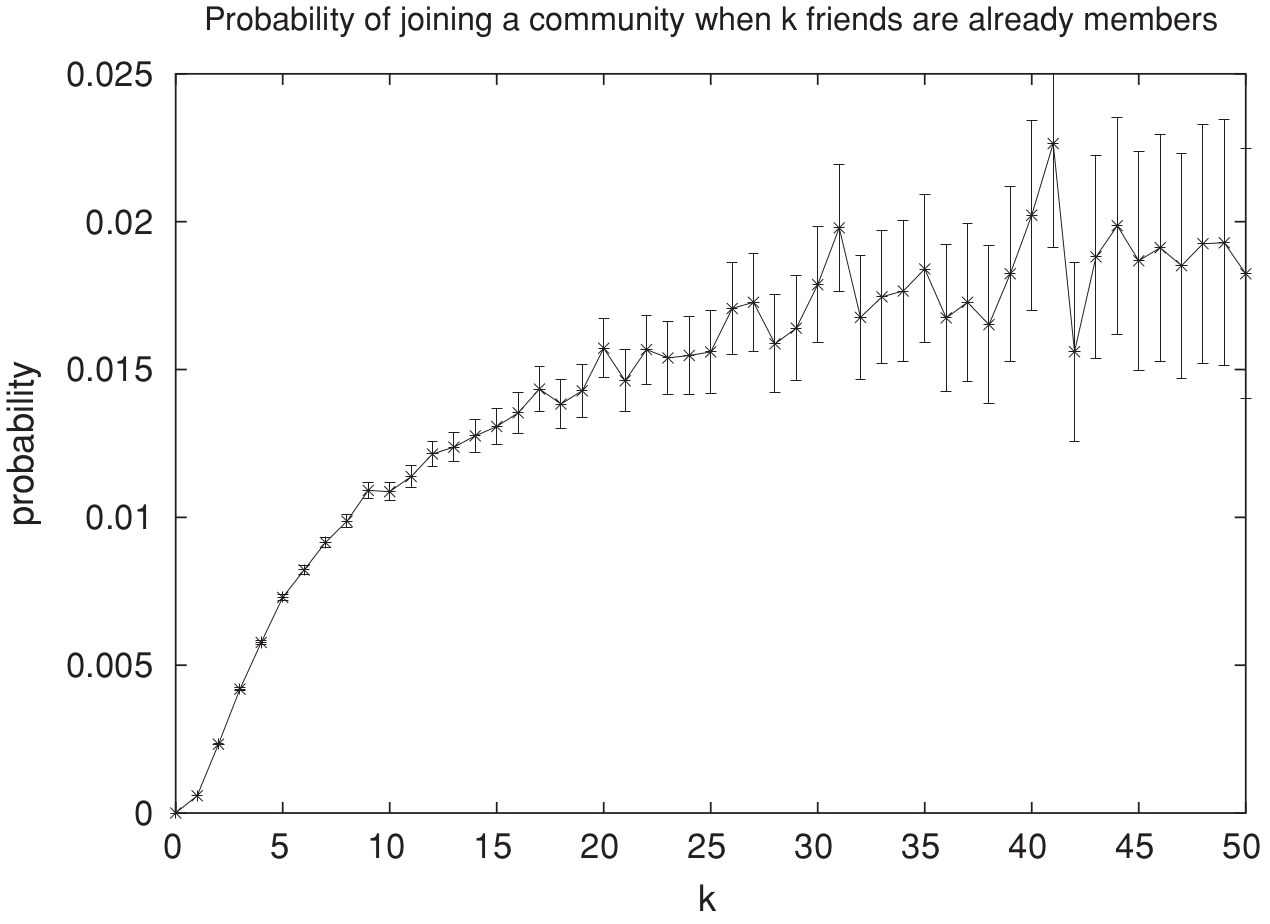
\includegraphics[width=\textwidth]{images/21_community.png}
    \caption{Quantification des effets de la fermeture d'adhésion dans
        un large ensemble de données en ligne : Le graphe montre la
        probabilité de rejoindre une communauté LiveJournal en fonction
    du nombre d'amis qui sont déjà membres.}
    \label{community}
\end{figure}

Enfin, la figure \ref{community} (fermeture d'adhésion) présente aussi un saturation à partir d'un certains nombre d'amis qui ont le même point d'intérêt.

\clearpage

\section{Quantifier les rôles relatifs de sélection d'influence sociale}
Les mécanismes de similitude :
\begin{itemize}
\item La sélection (intérieur, c'est nous qui faisons le choix)
\item L'influence sociale (extérieur, c'est les autres qui nous influencent) 
\end{itemize}
\subsection{Comment quantifier cela ?}

\paragraph{Exemple - Wikipédia}
Il peut exister une similitude de comportement entre rédacteurs. Par exemple les articles sur lesquels ils travaillent.

Raisonnement :
\begin{itemize}
\item On a des rédacteurs
\item Un lien entre deux rédacteurs : ils communiquent par la "Talk page" (chaque article a une "Talk page"). Autrement dit, si un rédacteur B communique sur la page de A, alors il y a un lien.
\item Les "points d'intérêts" ici sont les articles.
\item Quantification de la similitude
	$$\displaystyle\frac{\mbox{nombre d'articles rédigés par A ET B}}{\mbox{nombre d'articles rédigés par A OU B}}$$
Notons dès lors que la similitude ne peut pas être plus petite que 0 ni plus grand que 1. $0 \leq sim \leq 1$
\item Le moment de rupture est le moment où le lien est créé.
\item On compare la similitude avant et après cette rupture (figure
    \ref{wikipedia}). C'est surtout la sélection qui joue avant, car chaque rédacteur choisit ce qu'il doit ajouter ou modifier par rapport à ce qu'a mis l'autre rédacteur. Après la rupture, c'est principalement l'influence sociale qui entre en jeu car les deux rédacteurs mettent leurs idées en commun. %TODO utiliser plus la figure 4.13 pour cet exemple
\end{itemize}

\begin{figure}[!ht]
    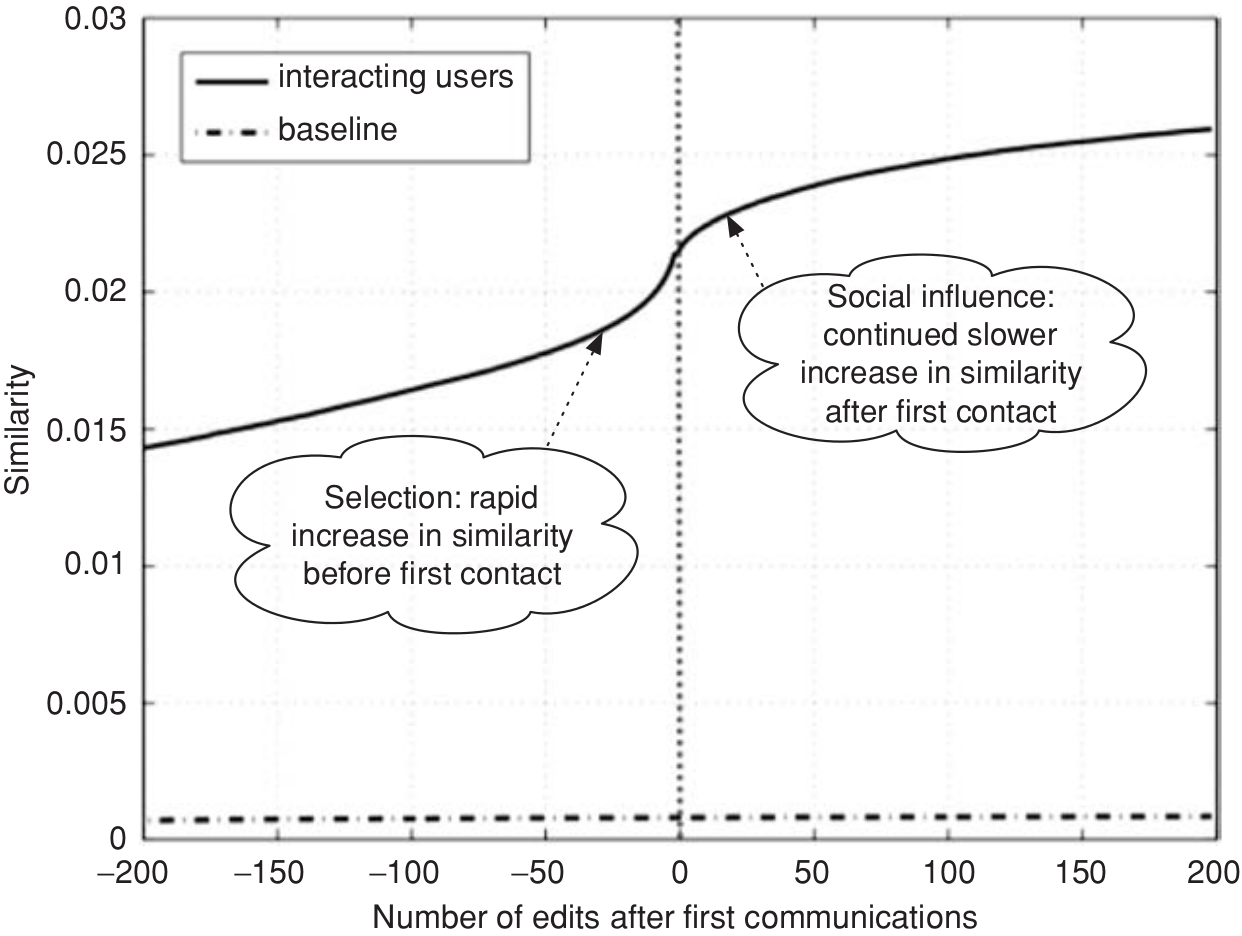
\includegraphics[width=\textwidth]{images/21_wikipedia.png}
    \caption{La similitude moyenne de deux contributeurs sur Wikipedia,
        relativement au temps (0) auquel ils ont communiqué pour la
        première fois. Le temps en abscisses, mesurés en unités
        discrètes correspond à une action Wikipedia faite par un des
        deux contributeurs. La courbe croît avant et après leur contact
        au temps 0, indiquant qu'à la fois la sélection et l'influence
        sociale joue un rôle ; la croissance de la similitude est plus
    forte juste avant le temps 0.}
    \label{wikipedia}
\end{figure}
